% !TEX program = xelatex

% Nejlepší zážitek zaručí:
%
% TeX distribuce: texlive-full
%
% Editor:
%   VS Code s doplňky
%       * LaTeX Workshop
%       * LaTeX Utilities
%       * Gnuplot
%
% Další závislosti:
%   latexmk
%   bibtex
%   gnuplot


% Jak používat:
% Zkompilovat: make
% Gnuplot: make gnuplot
% Vyčistit: make clean


% Základní balíčky
\documentclass[10pt,a4paper]{article}
\usepackage[utf8]{inputenc}
\usepackage[czech]{babel}
\usepackage{graphicx}
\usepackage{lmodern}
\usepackage{amsmath}
\usepackage[top = 2cm, bottom = 2cm, left = 2cm, right = 2cm]{geometry}

% Pro titulní stránku
\usepackage{titlesec}
\usepackage{setspace}
\usepackage{framed}
\usepackage{array}

% Vlastní balíčky 
\usepackage{gnuplottex}
\usepackage{epstopdf}
\usepackage{csvsimple}


\newcommand{\titjmeno}{Michal Grňo}
\newcommand{\titobor}{FOF}


\newcommand{\titcislo}{A7}
\newcommand{\titnazev}{Pozitronová emisní tomografie}
\newcommand{\titmereni}{7. 10. 2019}
\newcommand{\titodevzdani}{20. 10. 2019}


\begin{document}


\thispagestyle{empty}
\newgeometry{top = 2.5cm, bottom = 0cm, left = 2.5cm, right = 3cm}

{%T tomto je uzavřena celá titulka
%Tloušťka rámečku
\setlength{\fboxrule}{1.5pt}

\noindent
\framebox{
\begin{minipage}{\textwidth}
\setlength{\parindent}{17.62482 pt}
\phantom{d}

\begin{minipage}{0.6\textwidth}
{
\Large Kabinet výuky obecné fyziky, UK MFF\\
}
\vspace*{0.2cm}

{
\bfseries
\huge Fyzikální praktikum %ČÍSLO
}
\end{minipage}
\begin{minipage}{0.4\textwidth}
\begin{center}
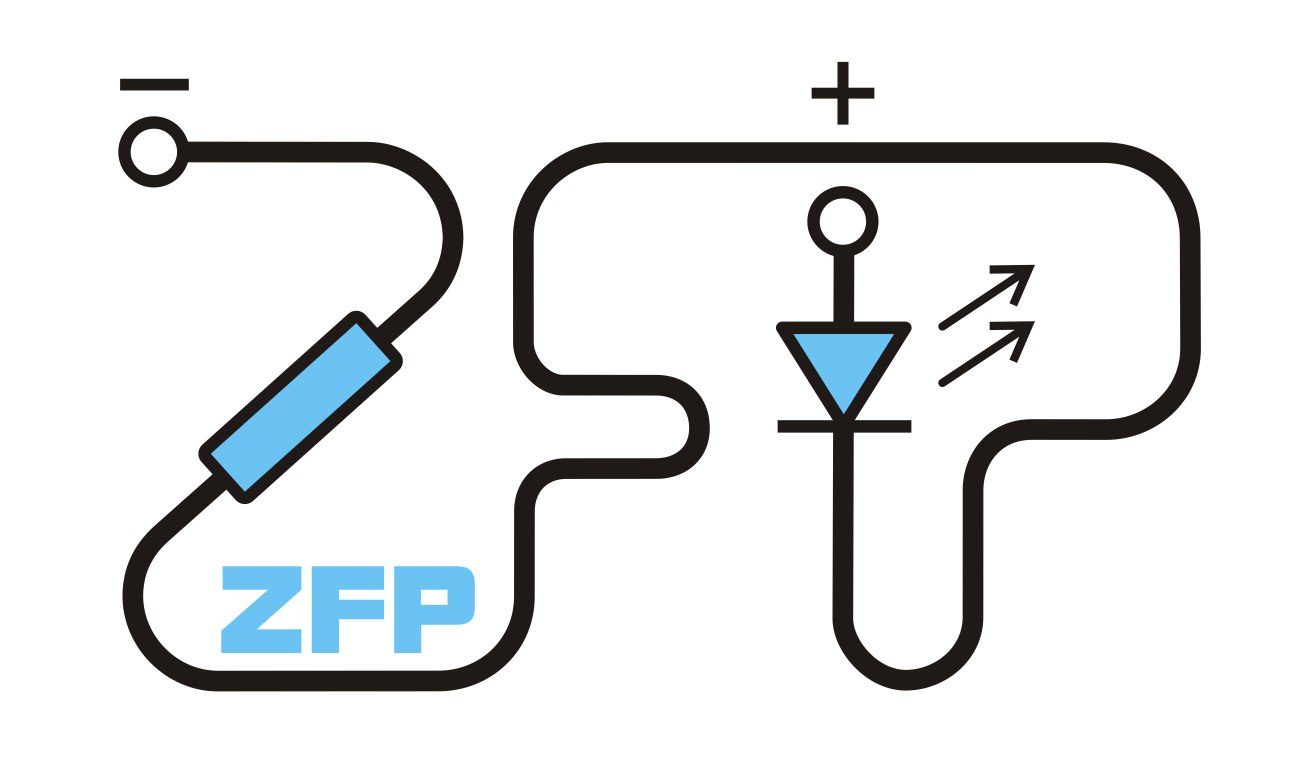
\includegraphics[width=4.5cm]{ZFP.jpg}
\end{center}
\end{minipage}\\\\

%\vspace*{0.5cm}

{
\setstretch{1.5}
\Large
\noindent
Úloha č. \titcislo

\noindent
Název úlohy: \titnazev

\noindent
Jméno: \titjmeno
\hspace*{\fill}
Obor: \titobor

\noindent
Datum měření: \titmereni
\hspace*{\fill}
Datum odevzdání: \titodevzdani

\phantom{d}
}
\end{minipage}
}
%Konec horního rámečku

{
\phantom{d}

\Large
Připomínky opravujícího:\\
\vspace*{6.75cm}
}

\newcommand{\linka}{\noalign{\hrule height 1pt}}
\newcommand{\linkadva}{\noalign{\hrule height 1.5pt}}
\setlength\extrarowheight{9.5pt}
\Large
\noindent
\begin{tabular}{!{\vrule width 1.5pt} l !{\vrule width 1pt} c !{\vrule width 1pt} c !{\vrule width 1.5pt}}
\linkadva
   & Možný počet bodů & Udělený počet bodů \\\linkadva
  Práce při měření & 0-3 &  \\\linka
  Teoretická část & 0-2 &  \\\linka
  Výsledky a zpracování měření & 0-9 &  \\\linka
  Diskuse výsledků & 0-4 &  \\\linka
  Závěr & 0-1 &  \\\linka
  Použitá literatura & 0-1 &  \\\linkadva
  \hspace*{\fill} \textbf{Celkem} \hspace*{\fill}& max. 20 &  \\
\linkadva
\end{tabular}
\phantom{d}

Posuzoval: \hspace*{\fill}dne:~~~~~~~~~~~~~~~~~

}%Konec uzavření titulky
\newpage
\newgeometry{top = 2cm, bottom = 2cm, left = 2cm, right = 2cm}
\setcounter{page}{1}

\section{Pracovní úkoly}
\begin{enumerate}
    \item Poté, co vyučující umístí silnější zářič ${}^{22}$Na do stojánku, změřte úhlové rozdělení koincidencí v oblasti úhlů potřebné pro nalezení polohy zářiče, doba měření 20s. Vysvětlete tvar naměřeného úhlového rozdělení, získané poznatky využijte při domácím zpracování.

    \item Změřte četnost koincidencí pro úhly $\phi$ = 60°, 90°, 120° bez plechu a 120° s Pb plechem mezi detektory, doba měření 100s. Vysvětlete pozorované četnosti.
    
    \item Poté, co vyučující přidá do krabičky druhý zářič, změřte úhlové rozdělení koincidencí s krokem 5°.
    
    \item Zvolte aspoň 2 další vhodné úhly otočení krabičky $\psi$ a opakujte měření 3).
    
    \item Narýsujte přímky spojující detektory do obrázku připraveného u úlohy a odečtěte polohu průsečíku - polohu zářiče vůči krabičce. Pozn.: Při volbě otočení krabičky $\psi$ se můžete řídit polohou už zakreslených průsečíků.
    
    \item Vzdálenost detektoru od zářiče zakresleného na obrázku porovnejte s měřením skutečné vzdálenosti.
    
    \item Polohy zářičů vůči krabičce určujte pomocí vztahů a metod popsaných v návodu. Podle výsledků zpracování nakreslete obrázky analogické k obrázkům narýsoaným během praktika. Chyby polohy zářičů určete graficky
\end{enumerate}


\section{Teoretická část}
Teorie\cite{DUMMY:1}
\begin{equation*}
    A = 4
    \label{A}
\end{equation*}

\begin{figure}[h]
    \centering
    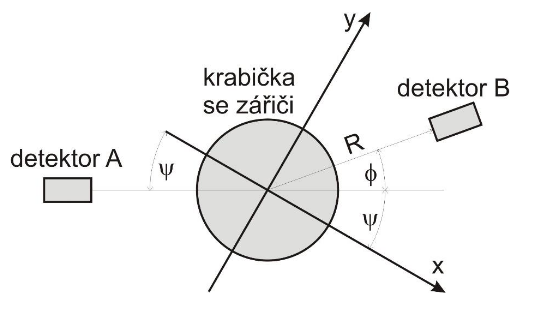
\includegraphics[width=10cm]{schema.png}
    \caption{Schéma koincidenčního měření, převzato z [1].}
\end{figure}


\section{Výsledky měření}
Naměřil jsem 3.


\begin{table}[h!]
    \centering
    \begin{tabular}{r|r|r}
        % Hlavička
        \bfseries $\psi$ &
        \bfseries $\varphi$ &
        \bfseries $\Delta\varphi$

        % Soubor
        % \csvreader[ head to column names ]{fits1.csv.tmp}{}
        % {
        %     \csviffirstrow{\\\hline}{\\} \psival\ & \phival & \phierr
        % }
    \end{tabular}

    \caption{Úhly získané regresí}
    \label{tab-fity-1vz}
\end{table}


\begin{table}[h!]
    \centering
    \begin{tabular}{r|r|r|r|r}
        % Hlavička
        \bfseries $\psi$ &
        \bfseries $\varphi_1$ &
        \bfseries $\Delta\varphi_1$ &
        \bfseries $\varphi_2$ &
        \bfseries $\Delta\varphi_2$

        % Soubor
        % \csvreader[ head to column names ]{fits3.csv.tmp}{}
        % {
        %     \csviffirstrow{\\\hline}{\\}
        %     \psival\ &
        %     \phiA & \phiAerr &
        %     \phiB & \phiBerr
        % }
    \end{tabular}
    
    \caption{Úhly získané regresí}
    \label{tab-fity-1vz}
\end{table}



\begin{figure}[p]
    \centering
    \begin{gnuplot}[terminal=epslatex,terminaloptions=color]
        plot 'data/CO_GRNO.PRN'
    \end{gnuplot}
\end{figure}


\section{Diskuse}
Bylo to špatně protože \eqref{A} 


\section{Závěr}
Bylo to hezké. assadfasd

\section{Literatura}
\bibliography{literatura} 
\bibliographystyle{ieeetr}

 
\end{document}